%% Included by 05-experiments.tex only when sections/phase-numbers.tex exists (E07 done).
\begin{figure}[t]
  \centering
  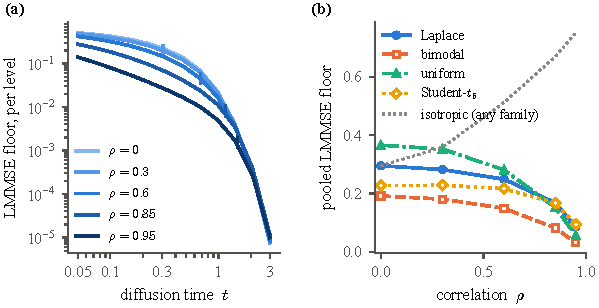
\includegraphics[width=\columnwidth]{fig_phase.pdf}
  \caption{\textbf{The second-order floor across correlation.} (a)~Per-level LMMSE
  floor on the Laplace chain for five $\corr$ (ticks: $\tstar(\corr)$); the floor
  collapses after the crossover. (b)~Schedule-pooled floor against $\corr$ for four
  innovation families, with the isotropic reference: strong correlation makes the score
  energy second-order-dominated, so the relative price of closure falls with $\corr$ while
  the absolute fourth-order structure does not.}
  \label{fig:phase}
\end{figure}
\paragraph{Across correlation.}
The floor is a function of the innovation law and of $\corr$ (\cref{fig:phase}): on the
Laplace chain it is $\phaseLmmseLaplaceRhozero$ for independent sites, $\phaseLmmseLaplaceRhozeropeightfive$
at the frozen $\corr=0.85$ and $\phaseLmmseLaplaceRhozeropninefive$ at $\corr=0.95$, where
$\tstar=\phaseTstarRhozeropninefive$ and the covariance carries most of the score energy
until late in the schedule. The families order by the size of their fourth cumulant at
every $\corr$; the isotropic reference rises with $\corr$ because the covariance itself is
what an unstructured estimator must learn first.
